\chapter{Precision frequency noise metrology of a superconducting qubit}

\section{Statement of the problem}
Relaxation processes characterized by $T_1$ represent one critical class of decoherence mechansims.
The resonator measurements of \rd{Ch TiN and ch Vortex} attempt to address this class of errors.
The other primary class of decoherence mechanisms are dephasing processes through which the relative phase of the superpositon state becomes increasingly uncertain are due to interaction with uncontrolled external degrees of freedom.
An important example of such a process is noise in the qubit frequency as it responds to randomly varying magnetic flux passing through the DC SQUID loop of our qubit.
As a first step to eliminating this flux noise in our device we wish to characterize the power spectral density (PSD) of this random process.
This power spectrum provides important information that can be used to identify the noise source and qualify our efforts to mitigate the noise.
%We can probe the noise mechanisms by probing the spectral character of the noise that they impart on the qubit.
\begin{figure}[h]
    \begin{center}
        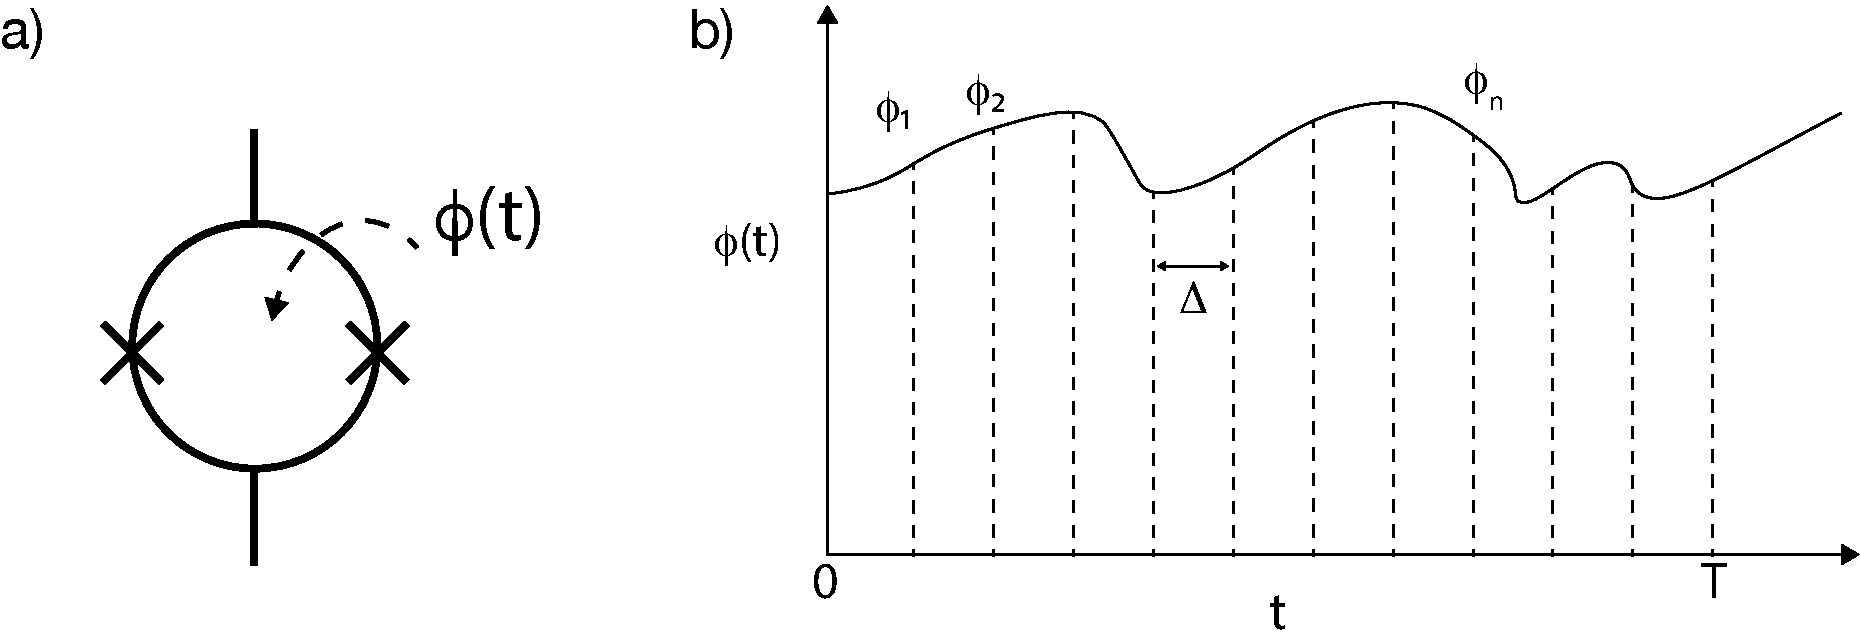
\includegraphics[width=150mm]{./PDF/flux_noise_schematic_191007_212p.pdf}
    \end{center}
    \caption{\textbf{Flux noise schematic}
    a) Magnetic flux of magnitude $\phi$ threading a SQUID loop thereby changing the effective critical current.
    b) The continuous time random process $\phi (t)$ sampled at times $t_n$ to form a time series.
    c) Ensemble averaged switching probablity vs time in the experiment.
    d) The single shot record from sampling $\phi (t)$ with a qubit}
    \label{Averaging_window_size}
\end{figure}

Time series methods are a common approach to measuring the PSD, which is obtained from the autocorrelation of the qubit frequency.
An early and conceptually straight-forward implementation of this idea is the Ramsey tomography oscilloscope (RTO). \rd{Cite Dan}
In this method, we ensemble average repeated trials of a Ramsey measurement at fixed Ramsey delay to make a time series of the accumulated phase $\theta$.
The drawback of this implementation is that the large number of trials required to estimate $\theta$ results in a relatively low Nyquist frequency.
An improvement on the (RTO) is the single shot Ramsey tomography oscilloscope (SSRTO) method \rd{Cite Fei Yan}
which allows us to increase the Nyquist frequency of our spectrum to the reset time of our system.
The work in this chapter improves on this technique by eliminating the reset portion of the algorithm entirely.
This increases the Nyquist frequency of the single shot Ramsey technique by two orders of magnitude since the repetition rate is then limited by the duration of the readout pulse $\sim 1 \mu s$ rather than the qubit reset time $\sim 5 T_1 \approx 100 \mu s$.
We also demonstrate the calibration of the technique and show that it is reliable at the 20\% level.

\rd{Tie the flux power back to gate error via Peter's paper}
\rd{Can also cite Riste}\\
\rd{Can site a variety of other works on Noise if we want to really extend this chapter.}

\section{The single shot Ramsey technique}

\subsection{March meeting slides}
\begin{figure}[h]
    \begin{center}
    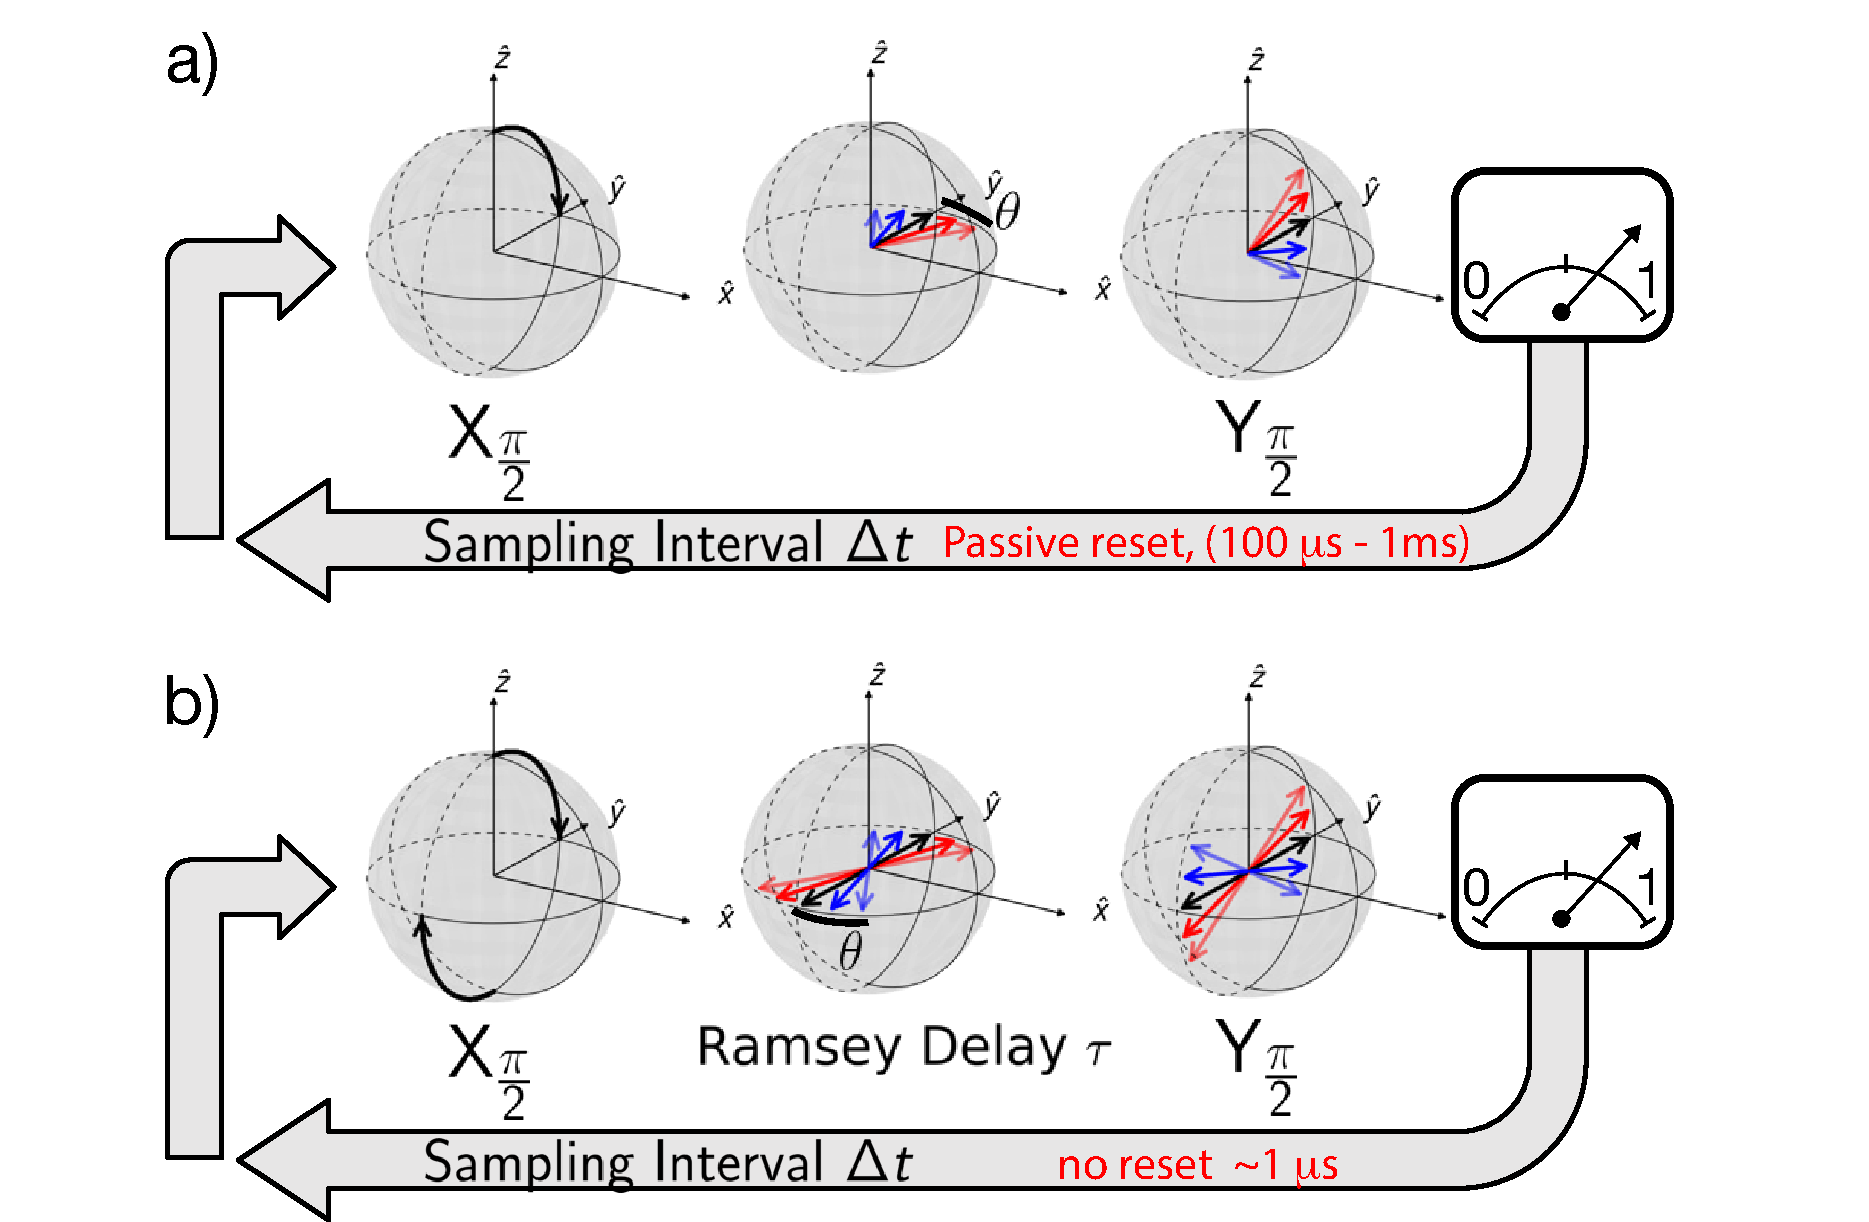
\includegraphics[width=175mm]{./PDF/ssrto_schematic_191001_646p.pdf}
    \end{center}
    \caption{\textbf{Schematic RTO}
    a) Schmatic diagram for the single shot Ramsey measurement.
    We first initialize the qubit into a phase sensitive superpositon state by doing an X/2 rotation.
    Next we allow the qubit to accumulate phase relative to the rotating frame.
    we then perform a Y/2 rotation to rotate the distribution onto the quantization axis.
    Finally, we project the qubit into either the $\ket{1}$ or $\ket{0}$.
    Afterword we wait on the order of 5 T1 for the qubit to relax to the ground state and repeat the measurement.
    b) The rapid SSRTO differs from the conventional SSRTO in a) in that the reset phase has been eliminated and the initial state may be either $\ket{0}$ or $\ket{1}$
    }
    \label{SSRTO Schematic}
\end{figure}

\subsection{mathematical derivation \rd{cite Dan unpublished and Fei}}

The magnetic flux threading the qubit loop is a continuous time random process $\phi (t)$.
We model this as a wide-sense stationary process which has some useful mathematical properties.
The mean and variance of the distribution from which $\phi$ is drawn are time independent.
Further, autocorrelation and autocovariance are functions only of the time delay and not the absolute position in time.

We wish to estimate the power spectrum of $\phi (t)$ because for example this information can be used to clarify the source of the noise.

The Weiner-Khinchin theorem states that the power spectrum of a WSS process is the Fourier Transform of its autocorrelation function.

\begin{equation}
    \mathcal{S}(f) = \int_{-\infty}^{\infty} r_{xx} (\Delta) e^{- i 2 \pi f \Delta} d\Delta
\end{equation}

The autocorrelation is defined as the expectation value of the self correlation at time delay $\Delta$
\begin{equation}
    r_{xx} = \langle X(t) X(t+\Delta) \rangle
\end{equation}

For the discrete sampling case \rd{cite wikipedia spectral density, or...}
\begin{equation}
    S_{\omega} = \frac{\Delta}{N} \abs{\sum_n x_n e^{- i \omega n \Delta}}^2
\end{equation}

The quantum nature of our detector enters the picture here because it is a probabilistic detector where the Bernouli distribution depends on the angle $\theta$.
If during the ramsey delay, we accumulate a phase of $\theta$ after the second rotation, we will have
a probability of measuring $\ket{0}$ of $P_{\ket{0}} = \frac{1 + \sin (\theta)}{2}$
and probability of measuring $\ket{1}$ of $P_{\ket{1}} = \frac{1 + \sin (\theta)}{2}$
Taking this into account We can compute the expectation value explicitly:

If $\Delta \neq 0$

%\begin{cases}{\langle X^*_m X_n \rangle = 1}
%\begin{cases}{apple}
    %\text{probability (1,1)} & $\frac{1-\sin \theta_m}{2} \frac{1-\sin \theta_n}{2}$\\
    %\text{probability (0,0)} & $\frac{1+\sin \theta_m}{2} \frac{1+\sin \theta_n}{2}$
%\end{cases}

%\begin{cases}{$\langle X^*_m X_n \rangle = -1$}
    %\text{probability (1,0)} & $\frac{1-\sin \theta_m}{2} \frac{1+\sin \theta_n}{2}$\\
    %\text{probability (0,1)} & $\frac{1+\sin \theta_m}{2} \frac{1-\sin \theta_n}{2}$\\
%\end{cases}

\begin{eqnarray}
    \text{probability (1,1)}&=&\frac{1-\sin \theta_m}{2} \frac{1-\sin \theta_n}{2}\\
    \text{probability (0,0)}&=&\frac{1+\sin \theta_m}{2} \frac{1+\sin \theta_n}{2}\\
    \text{probability (1,0)}&=&\frac{1-\sin \theta_m}{2} \frac{1+\sin \theta_n}{2}\\
    \text{probability (0,1)}&=&\frac{1+\sin \theta_m}{2} \frac{1-\sin \theta_n}{2}\\
\end{eqnarray}
However if $\Delta=0$ there is perfect correlation.

Thus
\begin{equation}
\langle X^*_m X_n \rangle = (1 - \delta_nm) \sin{\theta_m} \sin{\theta_n} + \delta_{mn}
\end{equation}

\begin{figure}[h]
    \begin{center}
    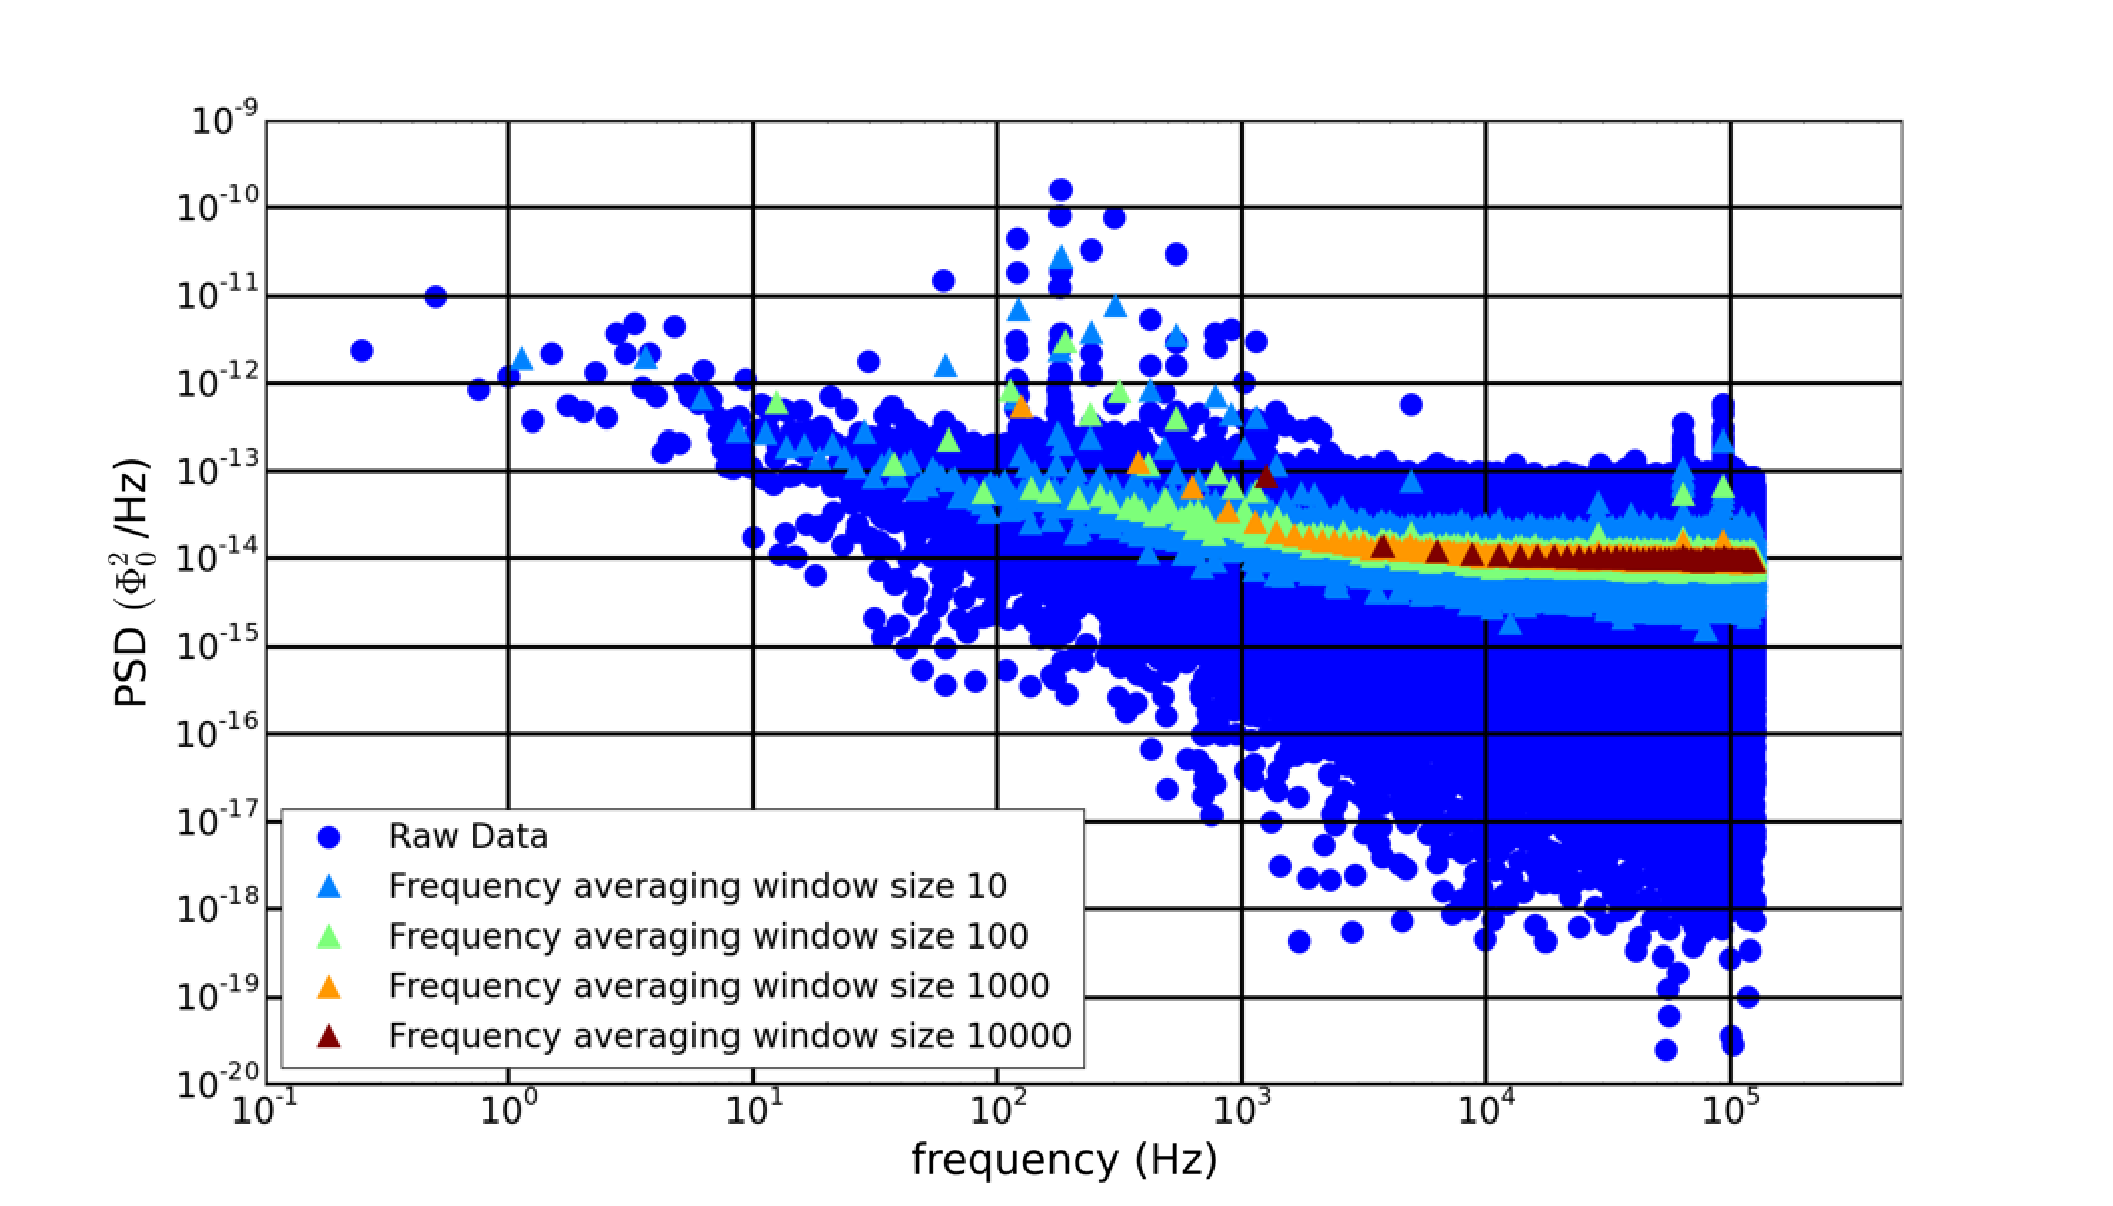
\includegraphics[width=175mm]{./PDF/averaging_window_size_191001_336p.pdf}
    \end{center}
    \caption{\textbf{Averaging adjacent frequencies}
    The Raw PSD data for all Fourier frequencies is shown in blue circles.
    The other colors show the average of adjacent Fourier frequencies within a the indicated window size}
    \label{Averaging_window_size}
\end{figure}

\begin{figure}[h]
    \begin{center}
    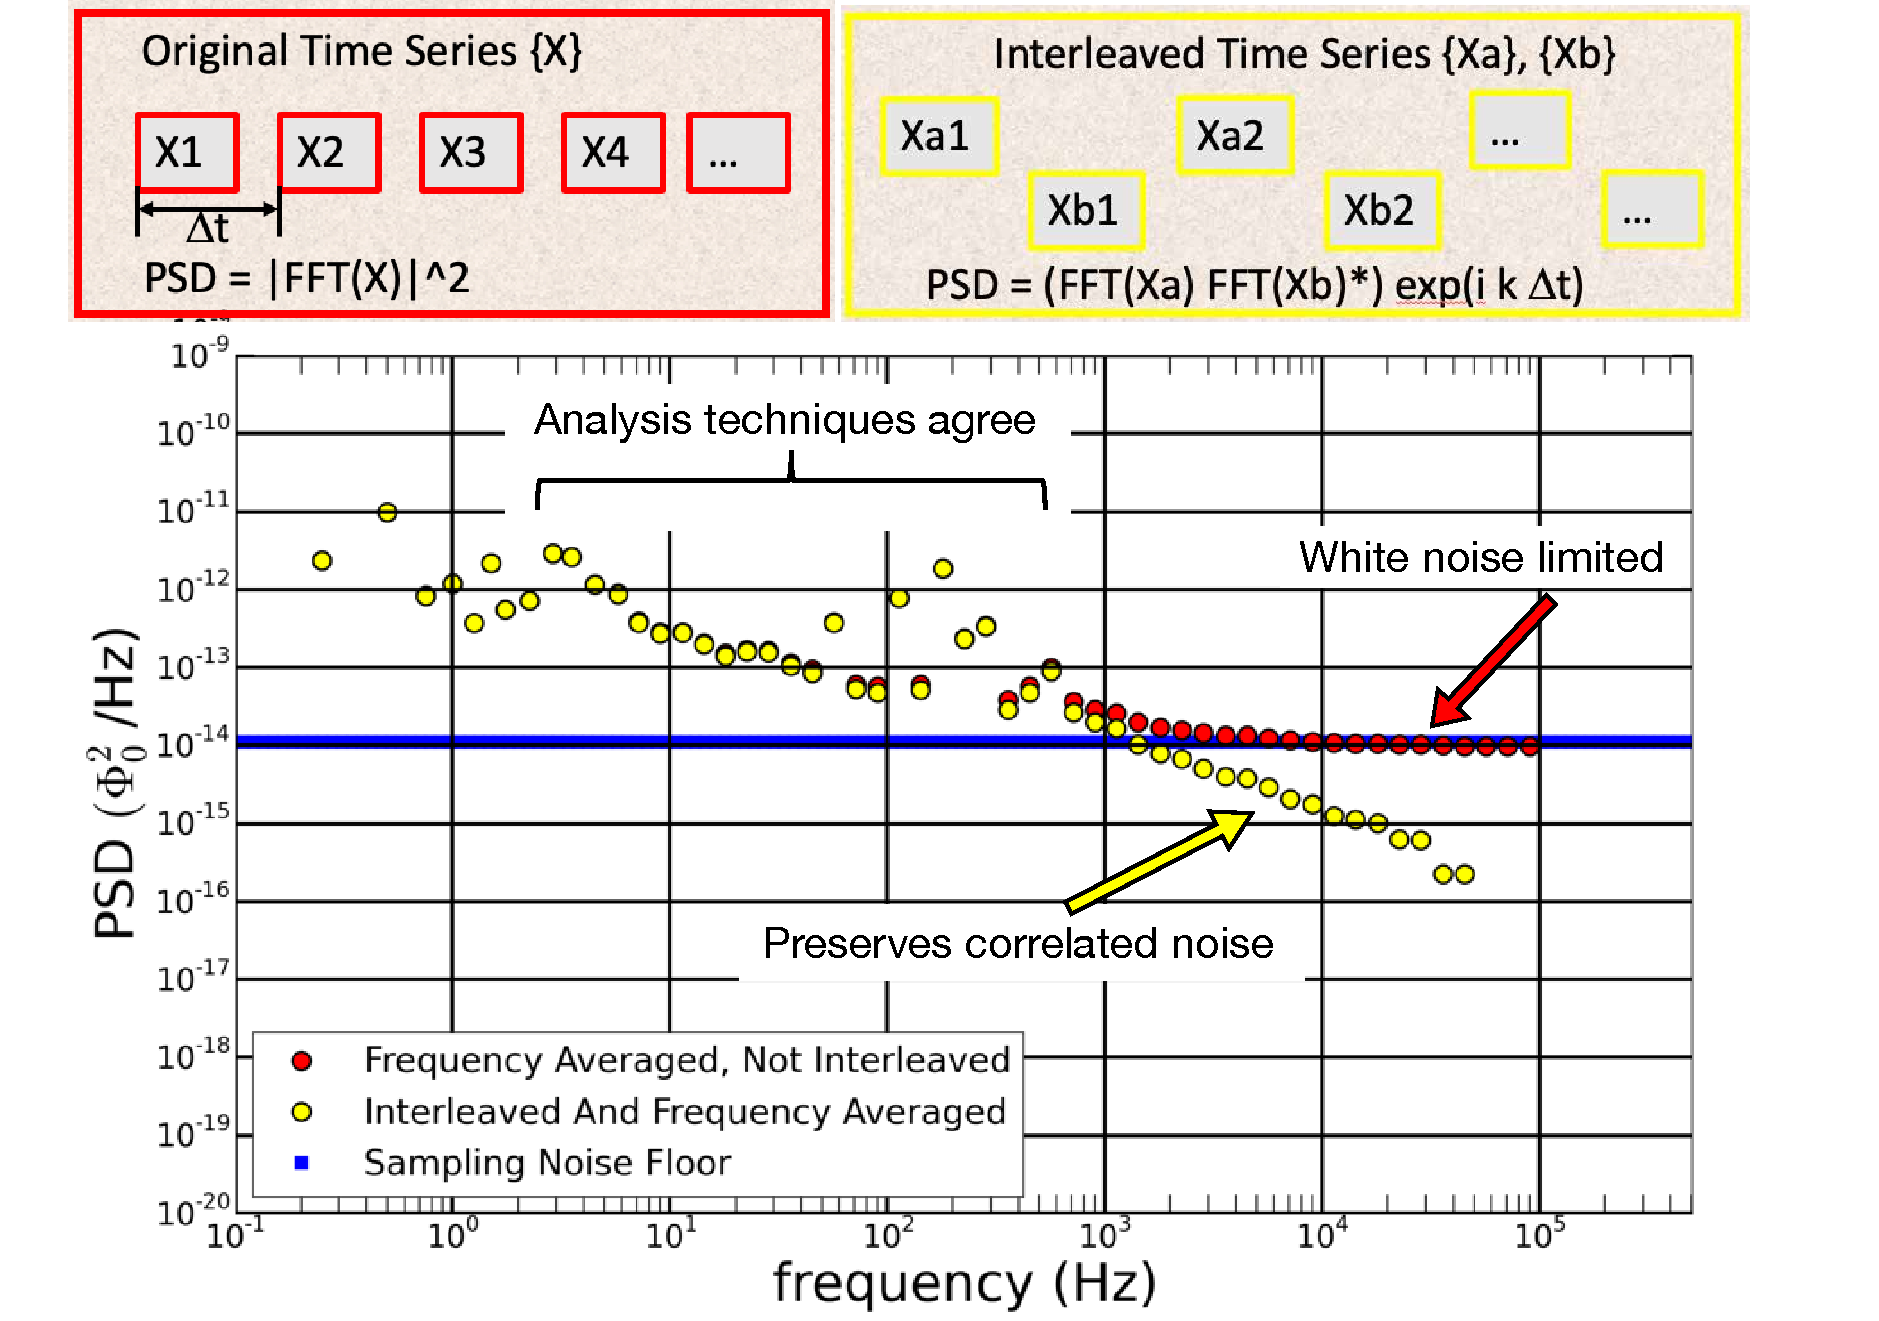
\includegraphics[width=175mm]{./PDF/interleaved_spectrum_191001_648p.pdf}
    \end{center}
    \caption{\textbf{Interleaved data processing}
    The PSD shown in red is the standard time series.
    The PSD shown in yellow is the result of interleaved data processing.
    At low frequencies above the white sampling noise floor the analysis techniques agree.
    At higher frequencies, the standard data processing technique is white noise limited.
    However, the interleaving procedure removes the white noise that is due to the zero delay term while preserving the correlated noise.
    }
    \label{Averaging_window_size}
\end{figure}

\begin{figure}[h]
    \begin{center}
        \hspace{-125mm}
    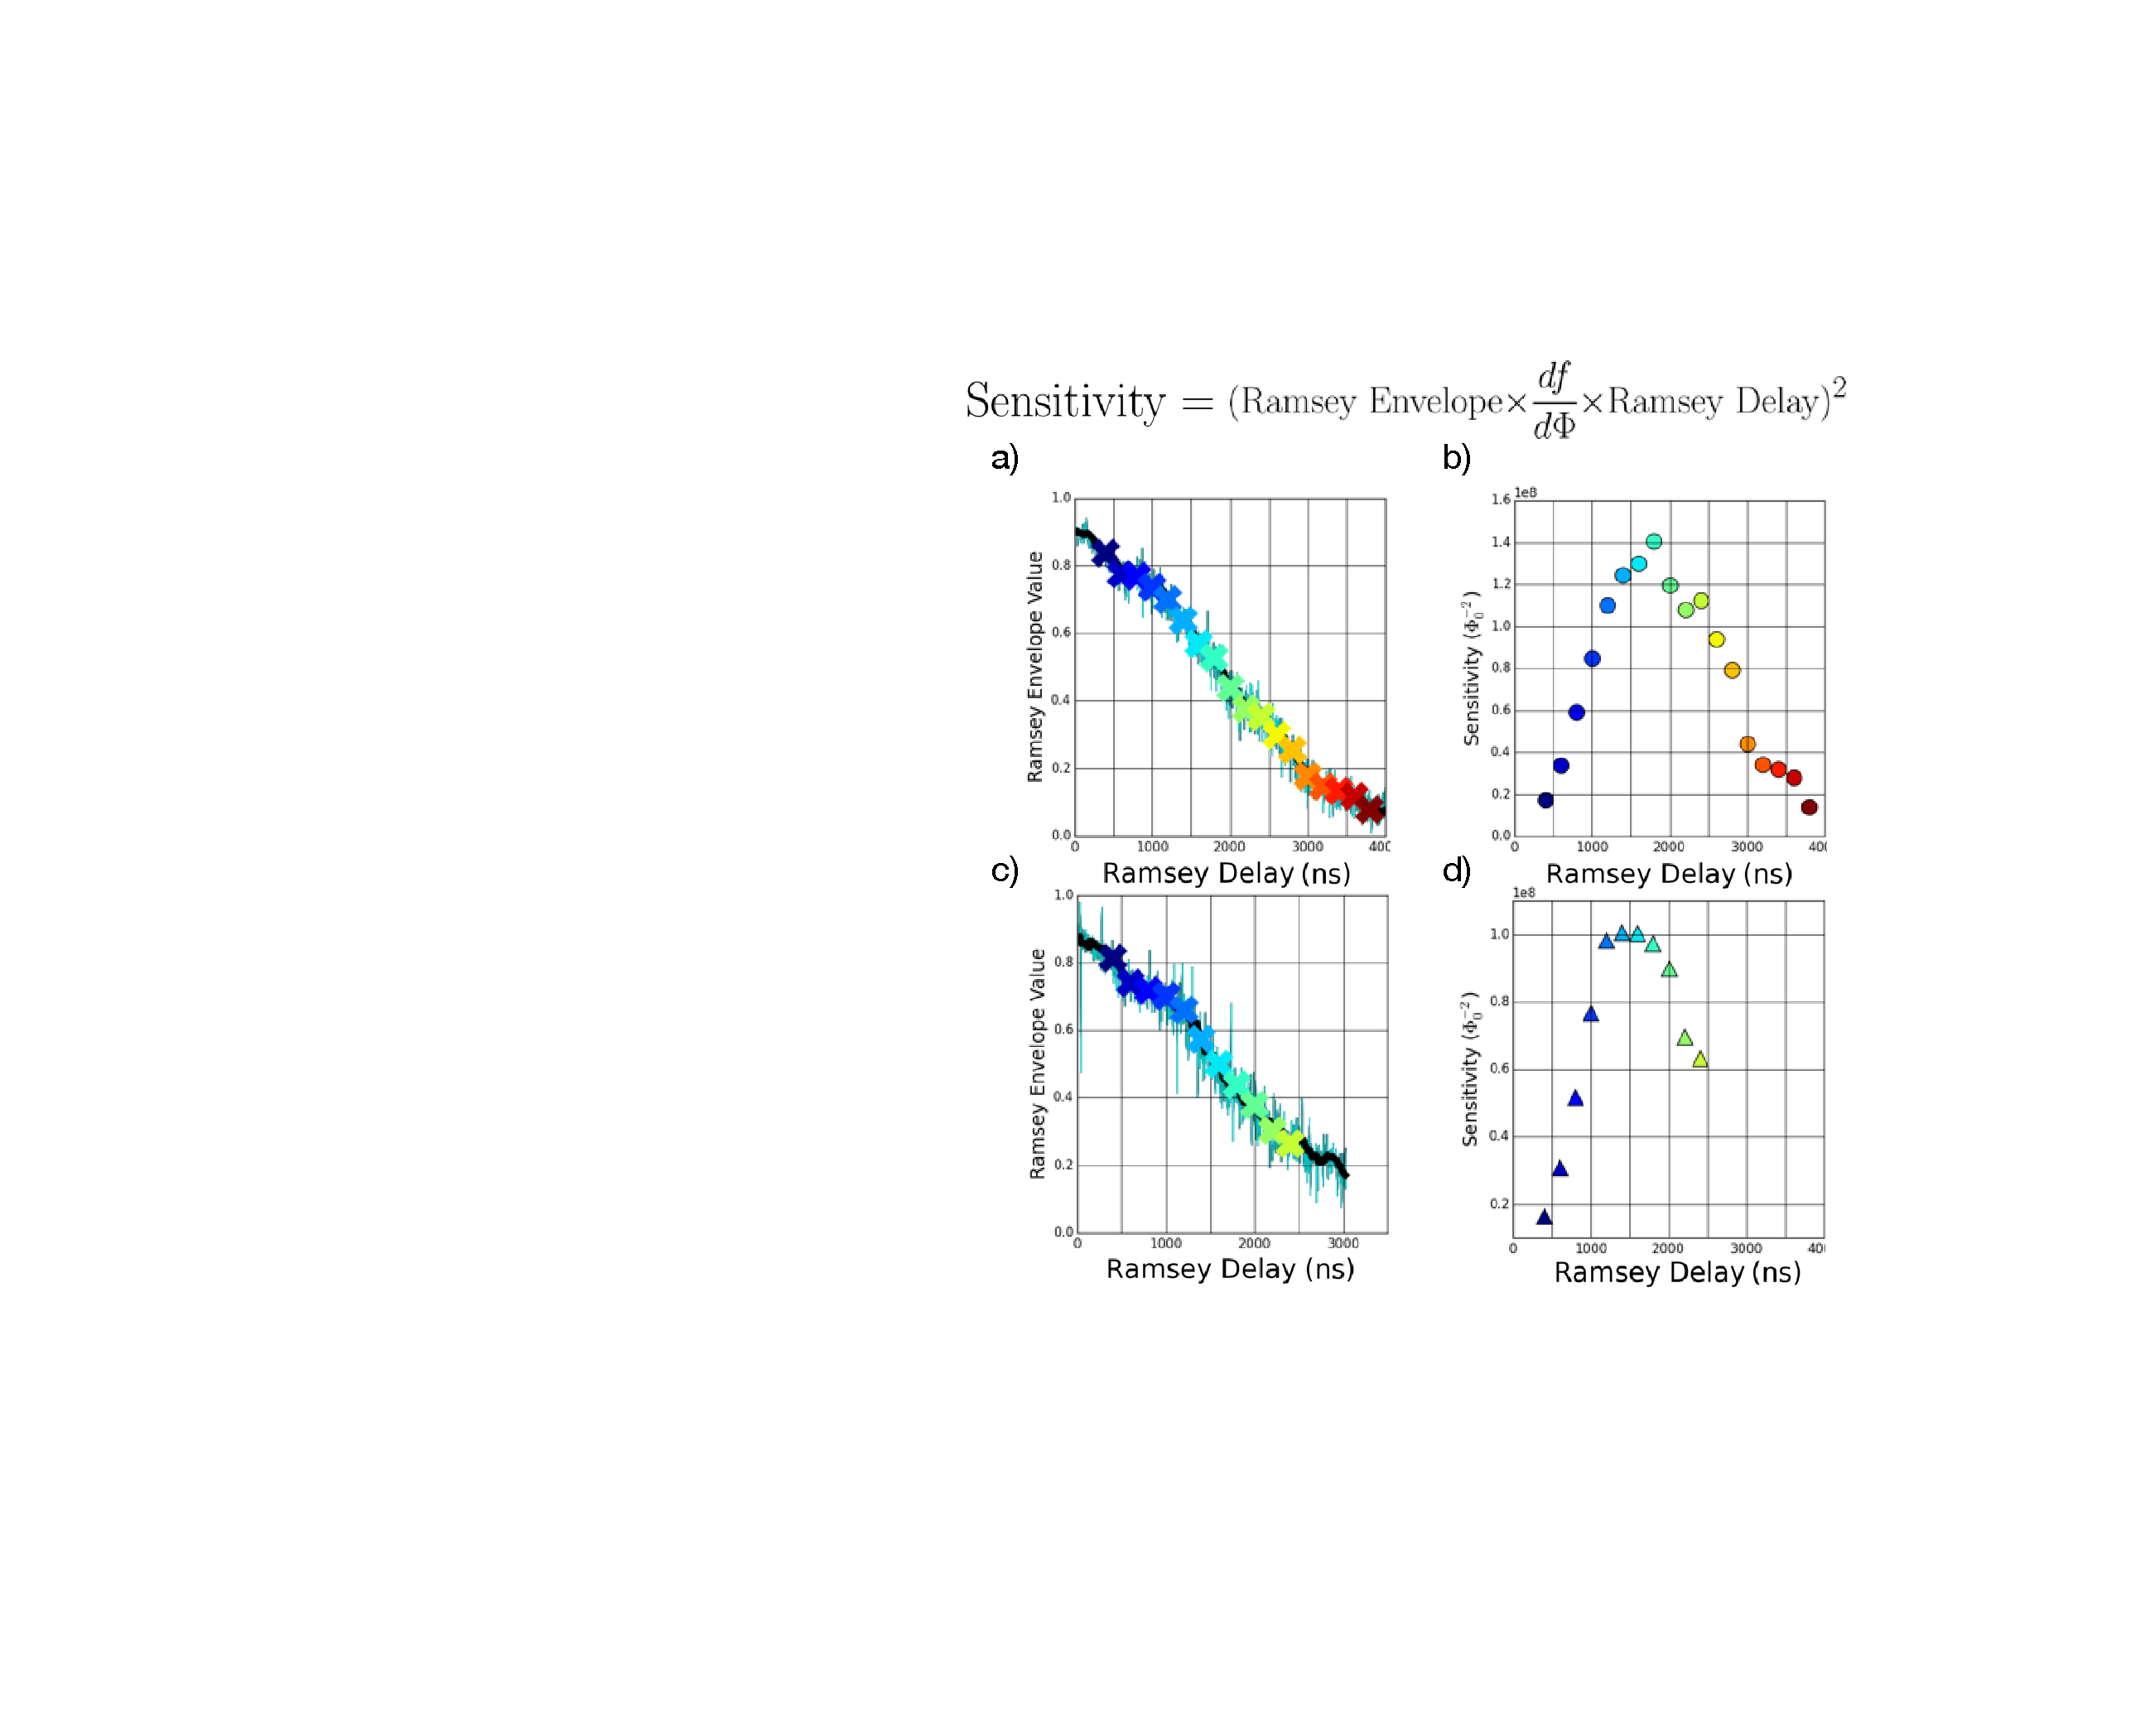
\includegraphics[width=275mm]{./PDF/sensitivity_vs_ramsey_delay_191001_649p.pdf}
    \end{center}
    \caption{\textbf{Sensitivity vs Ramsey delay}
    The conversion factor between the PSD of bits to a PSD of flux has three factors.
    The Ramsey delay, which is the ammount of time that the qubit acccumulates phase.
    The flux sensitivity, which converts a change in magnetic flux to a change in frequency.
    The the Ramsey envelope visibility, which is due to the fact that our qubit detector is not perfectly efficient.
    This is attributed to state preparation and measurement nonidealities and noise that is high frequency compared to the Ramsey delay time.
    }
    \label{SSRTO_sensitivity}
\end{figure}

\begin{figure}[h]
    \hspace{-65mm}
    \begin{center}
    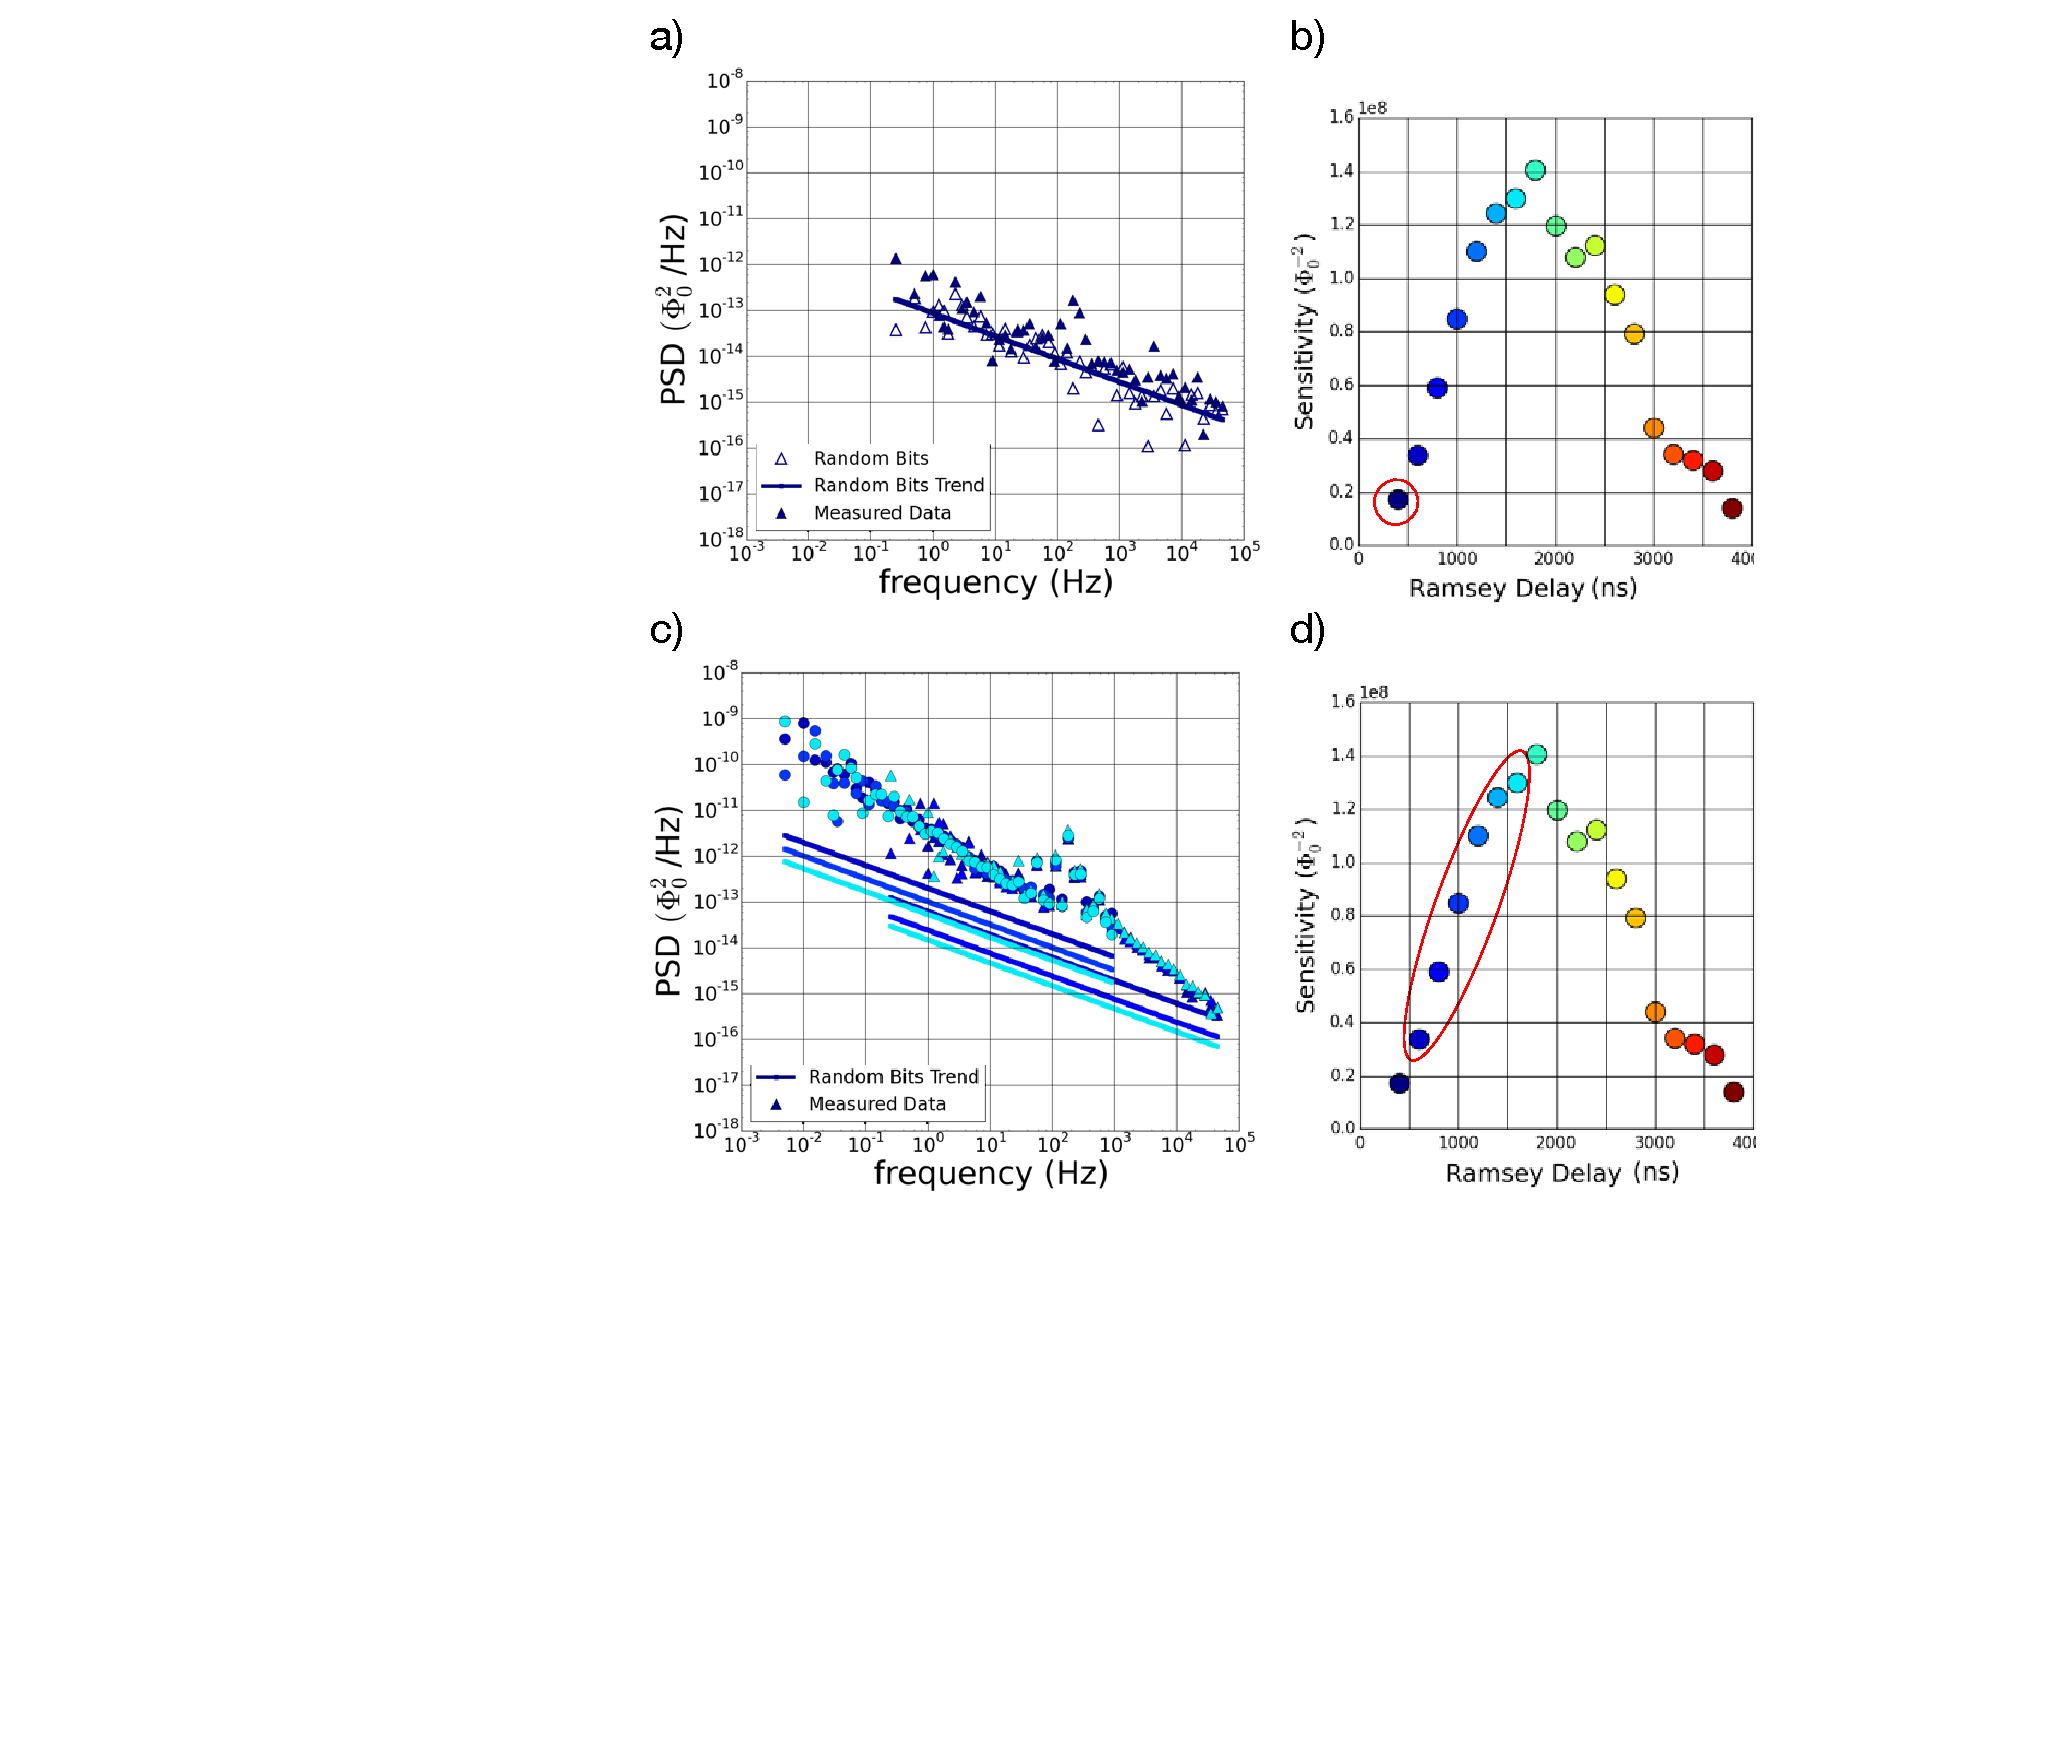
\includegraphics[width=225mm]{./PDF/random_bits_191001_649p.pdf}
    \end{center}
    \caption{\textbf{Random bits analysis verification}
    }
    \label{random_bits_calibration}
\end{figure}

\begin{figure}[h]
    \begin{center}
        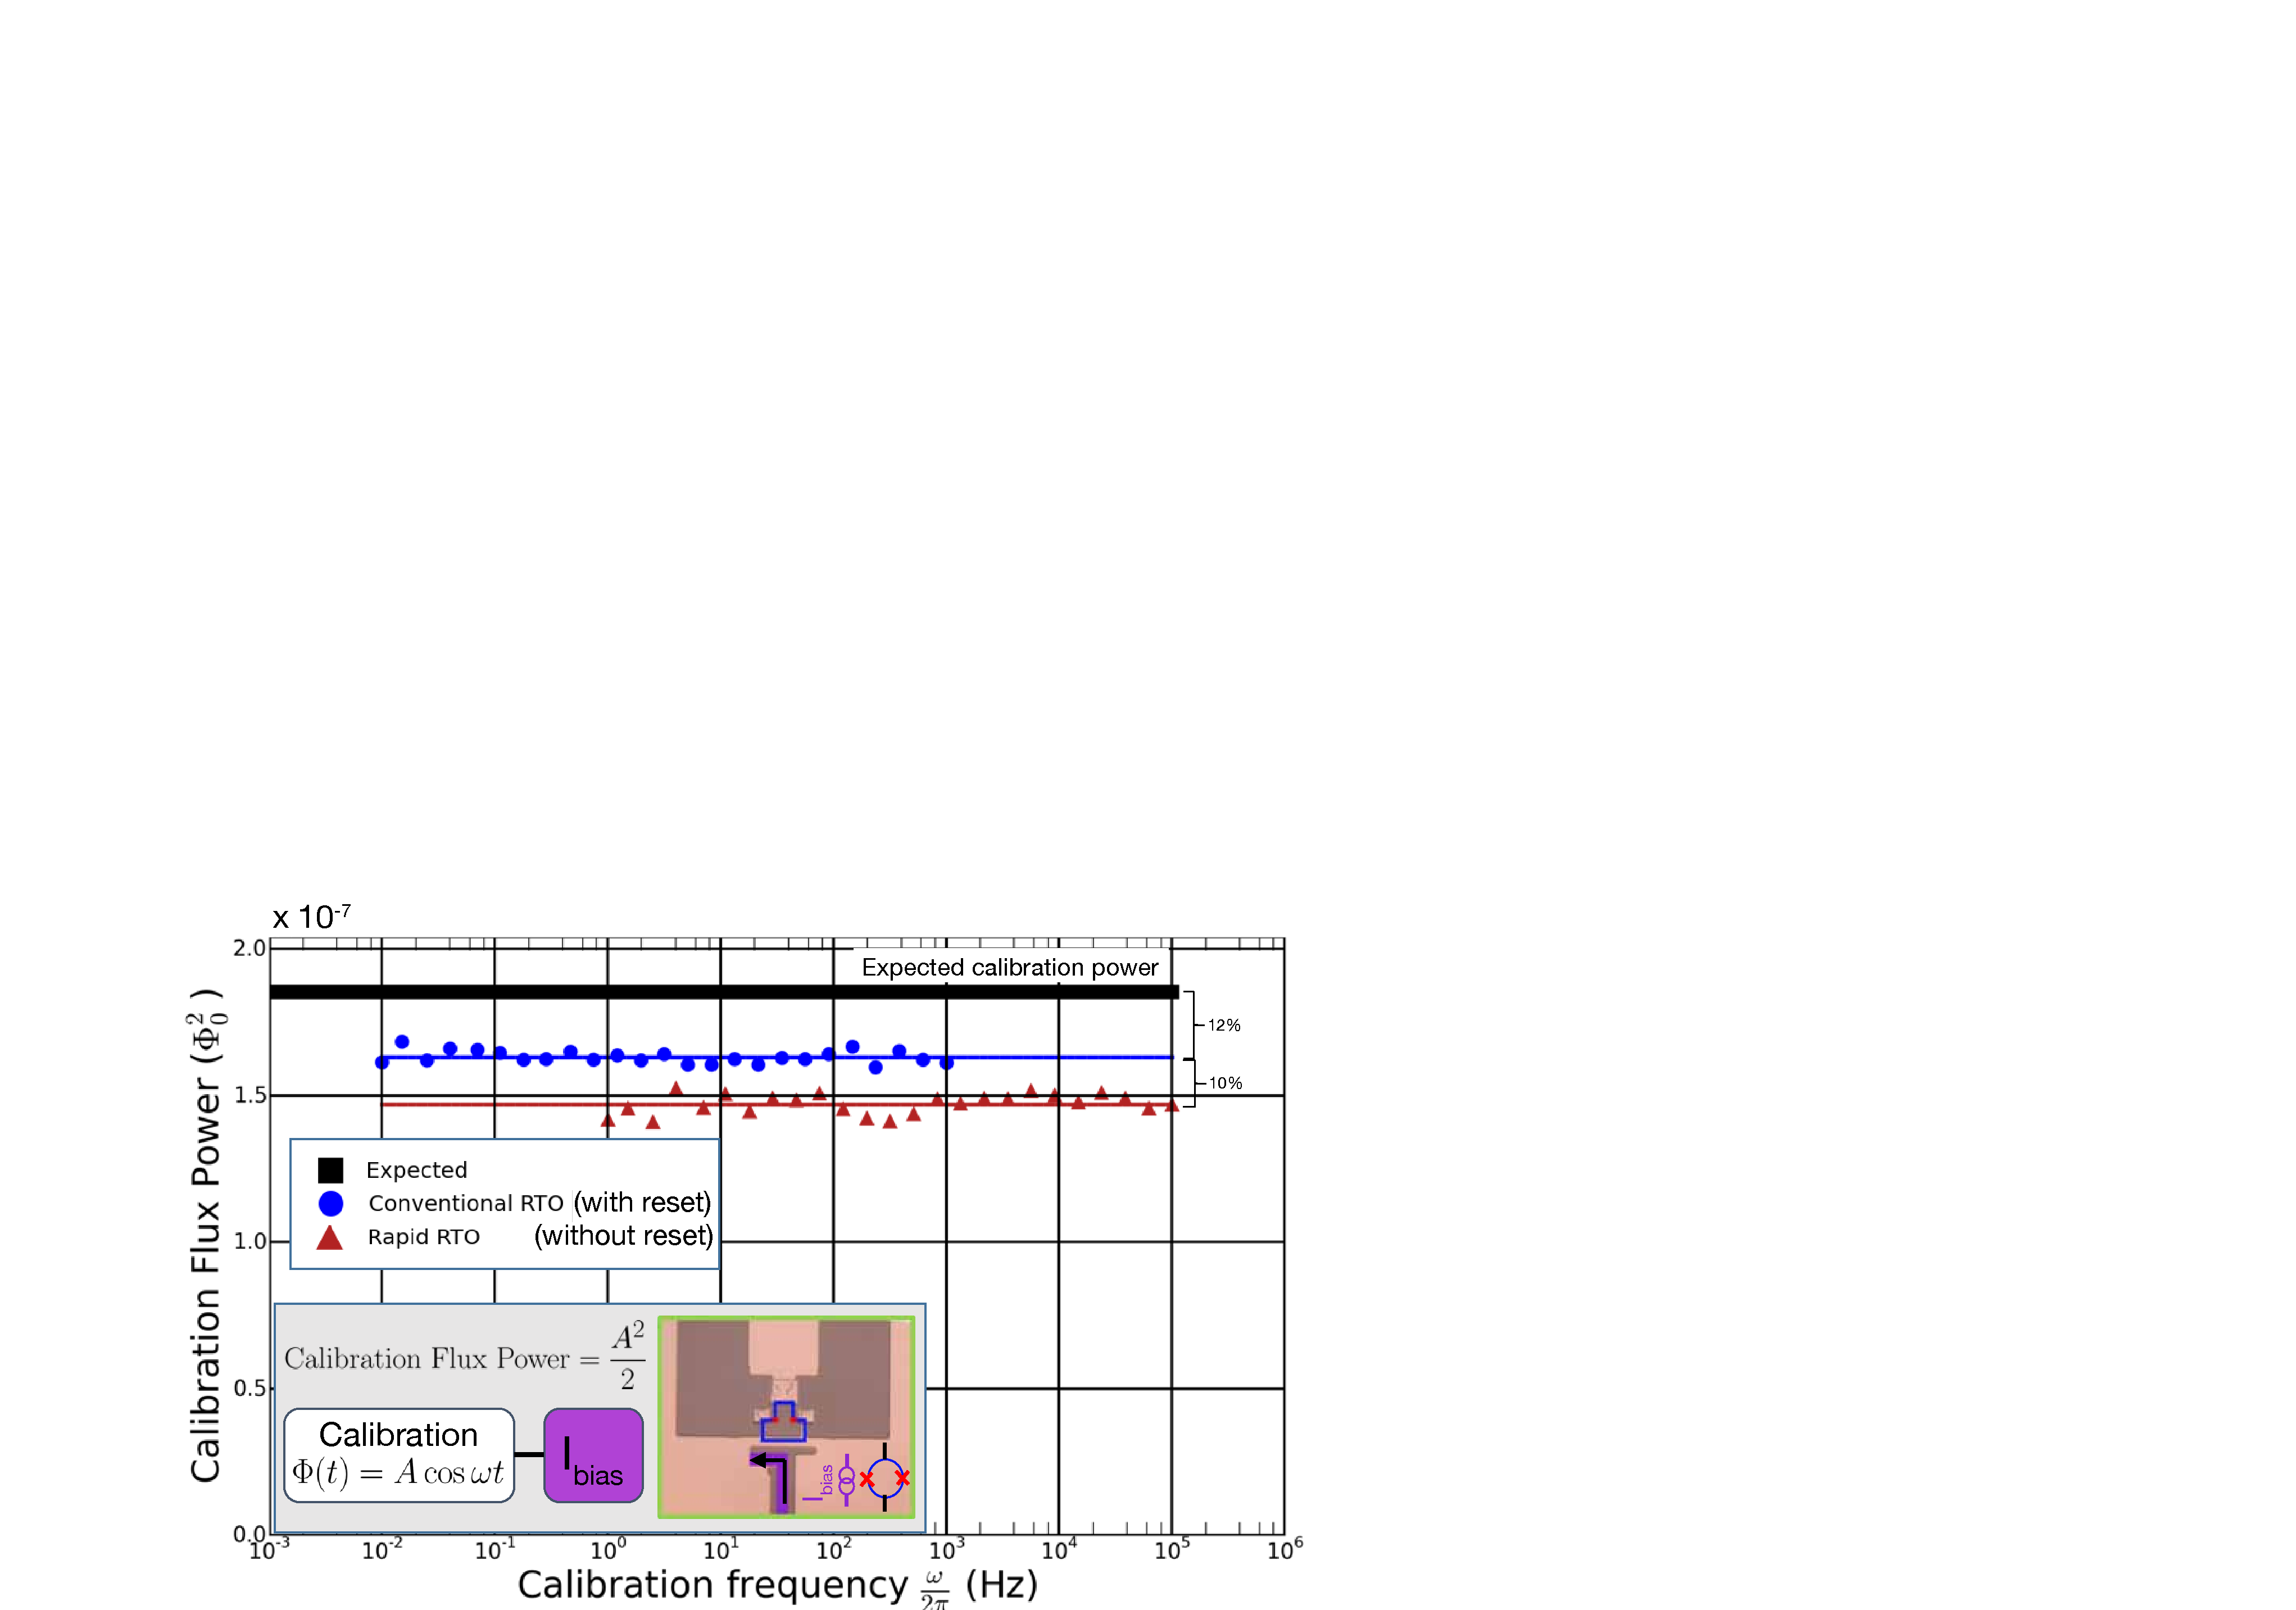
\includegraphics[width=300mm]{./PDF/coherent_tone_calibration_191001_650p.pdf}
    \end{center}
    \caption{\textbf{Coherent tone calibration}}
    \label{coherent_tone_calibration}
\end{figure}

\section{microwave bias T design}

\subimport*{./}{noiseCalBiasT_spec.tex}


